\section{基于概率的分类}
\label{sec:classification-probability}

第\ref{sec:classic-overview-probabilistic}节已区分直接建立条件类别概率与先描述类条件输入分布的两条路线。本节分别用Logistic回归、朴素贝叶斯和GDA说明参数估计、类别决策与概率检验。沿用训练集$D_n$，类别数为$C$、类别索引为$c$；$p$按观测类型表示概率质量函数或概率密度。LDA的共享协方差推导见第\ref{sec:classification-lda}节，这里直接在一般高斯模型族中使用该结果。

\subsection{Logistic 回归}
\label{sec:classification-logistic}

感知机与SVM用得分的正负决定类别，但有些任务还需要知道判断有多大把握。例如，把一封普通邮件误判为垃圾邮件，可能比让一封垃圾邮件进入收件箱更难接受。此时我们希望调整判为垃圾邮件的门槛，并用类别概率计算两种决定各自的预期代价。分类得分可以另行校准为概率，也可以从一开始就建立概率模型。

LDA能计算类别概率，但先要拟合每类的输入分布，这要求对“每类的输入长什么样”作出较强假设。这里改为直接描述$\mathbb P(Y=1\mid\bm X=\bm x)$：只关心给定输入后属于正类的概率，对输入本身如何分布不作假设。我们仍用特征的加权和组织证据，不过线性得分可能小于$0$或大于$1$，不能直接作为概率——把一个可能取$-3$或$5$的数解释成“概率”显然没有意义。\term{Logistic回归}（logistic regression）用一个S形函数把整条实数轴上的得分“压缩”到$(0,1)$区间，从而转成正类概率；它不要求输入服从类条件高斯分布，所规定的是对数几率与特征的线性关系。本节采用标签$\{0,1\}$，名称中的“回归”指概率与特征关系的建模。

第\ref{sec:regression-glm}节把伯努利分布、logit链接与其他响应模型统一在广义线性模型中；本节复用这套条件概率结构，但进一步规定类别决策阈值与误判代价，并单独检查概率校准。

\subsubsection{模型结构}
\label{sec:classification-logistic-structure}

记$p(\bm{x})=\mathbb{P}(y=1\mid\bm{x})$。比值$p(\bm{x})/[1-p(\bm{x})]$称为\term{几率}（odds），衡量正类相对于负类的可能性。对它取对数得到\term{对数几率}（log-odds，也称logit），其取值可以覆盖整个实数轴，因而适合与线性得分连接：
\begin{equation}
  \label{eq:classification-logistic-logodds}
  \log\frac{p(\bm{x})}{1-p(\bm{x})}
  =\bm{w}^{\top}\bm{x}+b.
\end{equation}
其中$\bm{w}\in\mathbb{R}^{d}$是权重，$b\in\mathbb{R}$是偏置。令右侧为$z$，由$p/(1-p)=e^z$整理出$p=e^z/(1+e^z)$，便得到
\begin{equation}
  \label{eq:classification-logistic-sigmoid}
  p(\bm{x})=\sigma(\bm{w}^{\top}\bm{x}+b),
  \qquad
  \sigma(z)=\frac{1}{1+e^{-z}}.
\end{equation}
这个S形函数称为\term{Sigmoid函数}（sigmoid function），此处特指Logistic形式。它把任意有限得分转成严格介于零和一之间的数。Cox在1958年的二值序列回归研究是这一统计建模路线的经典文献\scite{cox1958binary}。

参数的解释落在对数几率尺度上：保持其他特征不变，$x_j$增加一个单位，正类几率乘以$e^{w_j}$。概率本身的变化还取决于原来的概率，因为
\[
  \frac{\partial p(\bm{x})}{\partial x_j}
  =w_jp(\bm{x})[1-p(\bm{x})].
\]
在其余特征固定时，$w_j$的符号表示模型中正类对数几率的变化方向，大小则依赖特征单位。例如$w_j=\log 2$、原概率为$1/2$时，该特征增加一单位将几率乘以2，概率变为$2/3$。这种条件关联的因果解释还需要有关数据生成与混杂的额外假设。

在两类误判代价相同时，以$p(\bm{x})\geq1/2$预测正类，边界就是$\bm{w}^{\top}\bm{x}+b=0$。若误报的代价为$a>0$、漏报为$r>0$，正确分类代价为零，则预测正类的条件是$a[1-p(\bm{x})]\leq rp(\bm{x})$，即阈值改为$a/(a+r)$。这一决策解释要求输入概率足够可靠；可靠程度应通过与实际频率的比较检验。

图\ref{fig:classification-logistic-probability}把概率阈值与得分阈值放在同一条曲线上比较。一般地，概率阈值$\tau\in(0,1)$对应得分阈值$\log[\tau/(1-\tau)]$。在图中的教学设定下，误报与漏报代价相等时取$\tau=0.5$；若改成$a=4$、$r=1$，则$\tau=0.8$，得分至少达到$\log4\approx1.386$才预测正类。曲线本身没有改变，改变的是把概率转成类别的规则。
\begin{figure}[htbp]
  \centering
  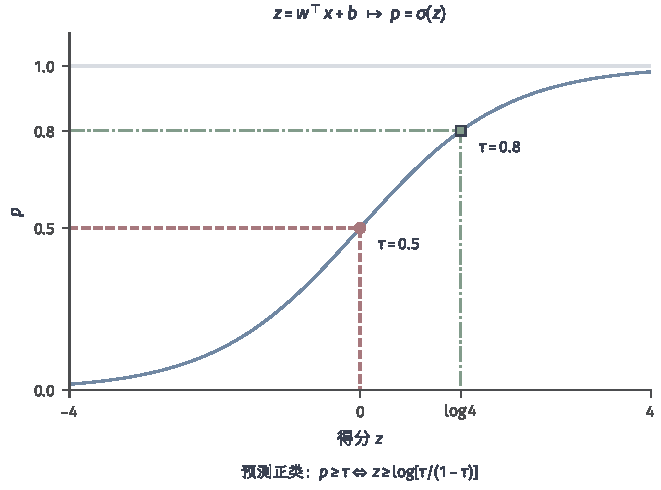
\includegraphics[width=105.412mm]{figures/04-classic-models/00-shared/matplotlib/classification-logistic-probability/figure.pdf}
  \caption{线性得分$z=\bm{w}^{\top}\bm{x}+b$经Logistic函数转为正类概率$p$。蓝色实线为$p=\sigma(z)$；红色虚线与圆点标出$(0,0.5)$，绿色点划线与方点标出$(\log4,0.8)$。两组辅助线分别连接概率阈值与对应的得分阈值，数值是教学构造，不表示训练或校准结果。}
  \label{fig:classification-logistic-probability}
\end{figure}

\subsubsection{参数学习}
\label{sec:classification-logistic-learning}

对独立样本，模型给出的标签概率为$p_i^{y_i}(1-p_i)^{1-y_i}$，其中$p_i=\sigma(\bm{w}^{\top}\bm{x}_i+b)$。\term{最大似然估计}（maximum likelihood estimation, MLE）选择使已观察标签最可能出现的参数。其条件对数似然为
\begin{equation}
  \label{eq:classification-logistic-likelihood}
  \ell(\bm{w},b)
  =\sum_{i=1}^{n}
  \bigl[y_i\log p_i+(1-y_i)\log(1-p_i)\bigr].
\end{equation}
最大化$\ell$等价于最小化负对数似然$L=-\ell$，也就是二分类\term{交叉熵损失}（cross-entropy loss）：给真实标签分配的概率越低，惩罚越大。令增广输入$\tilde{\bm{x}}_i=(\bm{x}_i^{\top},1)^{\top}$、参数$\bm{\beta}=(\bm{w}^{\top},b)^{\top}\in\mathbb{R}^{d+1}$，并记$z_i=\tilde{\bm{x}}_i^{\top}\bm{\beta}$，可写成
\begin{equation}
  \label{eq:classification-logistic-loss}
  L(\bm{\beta})
  =\sum_{i=1}^{n}\bigl[\log(1+e^{z_i})-y_i z_i\bigr].
\end{equation}
数值计算不宜先求极端概率再取对数，可用$\log(1+e^z)=\max\{0,z\}+\log(1+e^{-|z|})$避免指数溢出。

为确定更新方向，利用$\sigma'(z)=\sigma(z)[1-\sigma(z)]$求导。令$\tilde{\bm{X}}\in\mathbb{R}^{n\times(d+1)}$的第$i$行为$\tilde{\bm{x}}_i^{\top}$，$\bm{p}=(p_1,\ldots,p_n)^{\top}$、$\bm{y}=(y_1,\ldots,y_n)^{\top}$，则
\begin{equation}
  \label{eq:classification-logistic-derivatives}
  \begin{aligned}
    \nabla L(\bm{\beta})
      &=\tilde{\bm{X}}^{\top}(\bm{p}-\bm{y}),\\
    \nabla^2 L(\bm{\beta})
      &=\tilde{\bm{X}}^{\top}\bm{R}\tilde{\bm{X}},\\
    \bm{R}
      &=\operatorname{diag}\bigl(p_i(1-p_i)\bigr)_{i=1}^{n}.
  \end{aligned}
\end{equation}
梯度中的$p_i-y_i$是预测概率与观察标签的差。对任意$\bm{v}\in\mathbb{R}^{d+1}$，Hessian的二次型为
\[
  \bm{v}^{\top}\nabla^2L\,\bm{v}
  =\sum_{i=1}^{n}p_i(1-p_i)
    (\tilde{\bm{x}}_i^{\top}\bm{v})^2\geq0.
\]
所以负对数似然$L$是凸函数，而被最大化的$\ell$是凹函数。有限参数处的$p_i(1-p_i)>0$；若$\tilde{\bm{X}}$列满秩，$L$严格凸，否则可能存在不改变训练得分的平坦方向。这涉及\term{可识别性}（identifiability）：数据能否区分不同参数。即使严格凸，也只能保证有限极小点若存在便唯一，不能保证它一定存在。

例如，若存在$\bm{\beta}_0$使$(2y_i-1)\tilde{\bm{x}}_i^{\top}\bm{\beta}_0>0$对所有样本成立，沿$t\bm{\beta}_0$令$t\to\infty$，每项损失均趋于零，但任意有限$t$的损失仍大于零。完全分离的数据因此没有有限MLE；准完全分离也可能使部分参数发散。完整的存在性分析需要区分分离、准分离和重叠情形\scite{albert1984existence}。

实际训练常加入$\lambda\lVert\bm{w}\rVert_2^2/2$，其中$\lambda>0$。这个$L_2$惩罚抑制权重无限增大，也改善病态方向的数值条件。若两类均有样本，所有权重都受惩罚而偏置不受惩罚，所得二分类目标仍有唯一有限极小点；但若训练集只有一类，偏置仍可独自趋于无穷。若连偏置也作正的二次惩罚，则整个增广参数方向都受约束。使用$\lambda\lVert\bm{w}\rVert_1$可得到稀疏权重，但目标不再处处可微，需要适合非光滑目标的求解步骤。

求解器的选择取决于数据规模和存储成本。稠密数据的一轮完整梯度计算为$O(nd)$，构造Hessian约为$O(nd^2)$，直接分解又需要$O(d^3)$。若存储$d\times d$量级的Hessian过于昂贵，\term{有限内存拟牛顿法}（limited-memory BFGS, L-BFGS）只保留少量历史更新来近似二阶信息。大规模稀疏数据则可采用\term{随机梯度下降}（stochastic gradient descent, SGD），每次用一个样本或小批量近似完整梯度。样本数、稀疏程度和精度要求共同决定求解选择。

中小规模问题还可用牛顿法。把正则项加入梯度与Hessian后，每轮解$\bm H_t\bm d_t=-\nabla F(\bm\beta^{(t)})$，再以带阻尼的$\bm\beta^{(t+1)}=\bm\beta^{(t)}+\eta_t\bm d_t$更新；$F$是当前受惩罚目标。第\ref{sec:regression-glm}节已把同一步改写成IRLS：按当前概率产生工作响应和权重，再解加权最小二乘。这里沿用其计算，不把工作响应误当作固定的新标签。实现应解线性方程而不显式求逆，并检查目标变化、梯度与预算；极端概率、病态设计或过大的完整牛顿步都需要数值处理。

\paragraph{多类概率的表示与学习}

\label{sec:classification-logistic-softmax}

从垃圾邮件判断转到新闻主题分类，候选类别可以是体育、科技、文化等多个互斥主题。若分别训练“是否属于某主题”的二分类概率模型，它们的输出未必相加等于$1$；同一篇新闻可能在多个模型中都得到较高概率。我们需要一个共同描述类别竞争的模型。\term{Softmax回归}（softmax regression，也称multinomial logistic regression）为每类建立一个得分，再通过共同分母把这些得分转成和为一的概率向量。其表示约束是任意两类的对数概率比为线性函数。

\textbf{模型结构。}为每类引入$\bm{w}_c\in\mathbb{R}^{d}$和$b_c\in\mathbb{R}$，令$z_c(\bm{x})=\bm{w}_c^{\top}\bm{x}+b_c$。其后验模型为
\begin{equation}
  \label{eq:classification-softmax-model}
  p_c(\bm{x})
  =\mathbb{P}(y=c\mid\bm{x})
  =\frac{\exp z_c(\bm{x})}
         {\sum_{r=1}^{C}\exp z_r(\bm{x})}.
\end{equation}
指数保证概率为正，分母保证归一化；两类之间的分母相消，得到
\[
  \log\frac{p_c(\bm{x})}{p_r(\bm{x})}
  =(\bm{w}_c-\bm{w}_r)^{\top}\bm{x}+b_c-b_r.
\]
当$C=2$时，$p_1(\bm{x})=\sigma((\bm{w}_1-\bm{w}_2)^{\top}\bm{x}+b_1-b_2)$。把第1类视为正类、第2类视为负类，就回到二分类Logistic回归。

共同增加得分不会改变概率。更具体地，对任意$\bm{a}\in\mathbb{R}^{d}$和$t\in\mathbb{R}$，变换$\bm{w}_c\mapsto\bm{w}_c+\bm{a}$、$b_c\mapsto b_c+t$使每个指数项同乘$\exp(\bm{a}^{\top}\bm{x}+t)$，因而全部约掉。这是$d+1$维的参数冗余。选择第$C$类为\term{参考类}（reference class），就是把该类完整的增广参数固定为零：
\begin{equation}
  \label{eq:classification-softmax-reference}
  \begin{gathered}
    \bm{w}_C=\bm{0},\qquad b_C=0,\\
    \log\frac{p_c(\bm{x})}{p_C(\bm{x})}
    =\bm{w}_c^{\top}\bm{x}+b_c
    \quad(c<C).
  \end{gathered}
\end{equation}
参考类约束需同时固定权重与偏置。$\lambda\sum_c\lVert\bm{w}_c\rVert_2^2/2$只消除共同权重平移，还须例如令$\sum_c b_c=0$或惩罚全部偏置，才能锁定共同偏置平移。参数冗余消除后，设计矩阵的秩决定数据能否区分剩余方向，数据分离则影响有限解的存在性。

\textbf{参数学习。}现在$y_i\in\{1,\ldots,C\}$，记$p_{i,c}=p_c(\bm{x}_i)$，$\bm{\Theta}\in\mathbb{R}^{(d+1)\times C}$的第$c$列为$\bm{\beta}_c=(\bm{w}_c^{\top},b_c)^{\top}$。多类负对数似然是
\begin{equation}
  \label{eq:classification-softmax-loss}
  \begin{aligned}
    L(\bm{\Theta})
      &=-\sum_{i=1}^{n}\log p_{i,y_i}\\
      &=\sum_{i=1}^{n}\left[
        \log\sum_{c=1}^{C}e^{z_c(\bm{x}_i)}
        -z_{y_i}(\bm{x}_i)\right].
  \end{aligned}
\end{equation}
多分类同样可以通过迭代优化学习参数。为构造每轮更新，先对上述损失求导；以$\mathbb{1}\{\cdot\}$表示条件成立时为一、否则为零的指示函数，得到
\begin{equation}
  \label{eq:classification-softmax-gradient}
  \begin{aligned}
    \nabla_{\bm{w}_c}L
      &=\sum_{i=1}^{n}
        [p_{i,c}-\mathbb{1}\{y_i=c\}]\bm{x}_i,\\
    \frac{\partial L}{\partial b_c}
      &=\sum_{i=1}^{n}
        [p_{i,c}-\mathbb{1}\{y_i=c\}].
  \end{aligned}
\end{equation}
梯度仍由“预测概率减观察标签”组成。目标凸，但共同参数平移及秩亏可能带来平坦方向，分离数据也可能没有有限MLE。参考类约束消除表示冗余，正则化控制参数大小，两者的作用不同。

Softmax可用分块牛顿法、L-BFGS或小批量SGD优化，多类Hessian还包含类别间的耦合，不能简单把$C$个独立的二分类IRLS问题拼起来。求概率时应先减去$m(\bm{x})=\max_c z_c(\bm{x})$，用$e^{z_c-m}/\sum_r e^{z_r-m}$得到完全相同且更稳定的结果。普通稠密实现的一轮梯度计算约为$O(ndC)$。

预测可取$\hat y(\bm{x})=\argmax_c p_c(\bm{x})=\argmax_c z_c(\bm{x})$，并按固定类别次序处理平局。共同分母不改变得分排序，所以只需输出一个类别时，可以直接比较各类得分。

\paragraph{交叉熵在拟合什么}
\label{sec:classification-logistic-theory}
记真实类别后验为$\bm\eta(\bm x)$，预测概率向量为$\bm p(\bm x)$。固定输入时，预测交叉熵减去真实后验的熵为
\[
 -\sum_c\eta_c\log p_c+\sum_c\eta_c\log\eta_c
 =D_{\mathrm{KL}}(\bm\eta\Vert\bm p)\geq0.
\]
因此最理想的条件概率目标是真实后验；使用有限参数的Logistic或Softmax时，只能在所设定的对数几率关系中拟合它。若目标的对数几率需要平方或交互项，应改变输入特征，而不是只增加优化轮数。分类又只取最大概率的类别，所以概率拟合误差与分类错误是不同的评价对象。

\subsubsection{概率校准与温度缩放}

\label{sec:classification-probability-calibration}

需要用概率设定邮件拦截门槛时，还要检查报告的置信度能否对应实际频率。Softmax输出满足概率公理，却不自动满足\term{概率校准}（probability calibration）。例如，在报告某类概率约为$0.8$的一组样本中，该类的实际比例也应接近$0.8$。有限样本、模型失配、正则化和分布变化都可能破坏这种对应。这里检验的是报告概率与实际频率的联系，和按最大概率选择类别是不同的问题。

一种简洁的后处理是温度缩放（temperature scaling）：固定已训练得分$z_c(\bm x)$，只学习$T>0$，令$\tilde p_c(\bm x)=\exp(z_c/T)/\sum_r\exp(z_r/T)$。用未参与原模型拟合的校准记录最小化这组概率的负对数似然，就可估计温度；随后还要在另一份独立数据上评价。正温度不改变最高得分类别，却会改变概率的集中程度。Guo等在其研究的网络和数据上比较了这类方法；单一温度不能保证修复所有概率失配\scite{guo2017calibration}。

\subsubsection{层次Softmax、NCE与负采样}

\paragraph{降低大类别集的概率计算成本}
\label{sec:classification-softmax-hierarchical}

类别特别多时，平坦Softmax要在分母中累加全部类别的指数得分。\term{层次Softmax}（hierarchical softmax）改用树上路径概率的乘积表示一个类别的概率，把一次类别选择拆成沿路径进行的条件选择。这改变了概率的参数化方式，计算某个类别概率时可以沿相应路径展开；类别怎样组织成树，也就成为模型设计的一部分。若需要全部类别概率，计算负担仍然存在，沿路径计算一个类别的概率也不等于已经找到了最高概率类别\scite{goodfellow2016}。

用四个类别构造一个二叉树例子，可以分别看清归一化和搜索。把类别1、2放在根的左子树，类别3、4放在右子树。固定当前输入，设根节点向左的条件概率为$0.6$、向右为$0.4$；到达左子树以后，两片叶的条件概率为$0.5,0.5$；到达右子树以后，两片叶的条件概率为$0.99,0.01$。于是
\[
  \begin{aligned}
    p_1&=0.6\times0.5=0.3,&
    p_2&=0.6\times0.5=0.3,\\
    p_3&=0.4\times0.99=0.396,&
    p_4&=0.4\times0.01=0.004.
  \end{aligned}
\]
四类概率相加为一，因为每个内部节点都把到达它的概率质量完整分给两个孩子。内部节点可以各用一个Logistic模型给出两条分支的条件概率；一旦指定叶子，只需计算沿途节点，不必访问无关分支。在平衡二叉树中，路径长度约为$\log_2C$，不平衡树的路径则可能更长。给定类别树后，一条训练记录的真实类别就确定沿途的二元分支标签；训练时把这些节点的Logistic对数概率相加，沿路径求梯度并更新节点参数，无须访问无关分支。树的安排固定了哪些类别共享前面的判断，需要作为模型结构选择。

这个例子还表明，根处贪心选择较大的左支会错过概率最大的第3类。因此，计算指定类别的概率、找最高概率类别与输出全部类别概率，是三种不同的计算任务。

\paragraph{减少显式归一化的训练负担}
\label{sec:classification-softmax-noise-contrast}

当归一化分母需要对大量候选求和时，也可以改变概率估计所用的训练问题。\term{噪声对比估计}（noise-contrastive estimation, NCE）通过区分数据与人为噪声来估计模型，训练时回答一条记录来自数据还是人为噪声，模型参数也决定这项区分的得分。归一化常数可以与模型参数一起估计，避免每一步都对全部候选得分显式求和。它与层次Softmax改变的位置不同：前者改变估计问题，后者把类别概率分解到树上，不能把两者都当作原平坦Softmax公式的计算改写\scite{goodfellow2016}。

沿用新闻主题分类，可以把这一辅助任务写出来。固定输入$\bm x$，原任务的随机变量$Y$仍表示新闻主题，真实后验为$\eta_c(\bm x)$。现在对每一条真实记录$(\bm x,c^+)$，从已知、可抽样且可求值的噪声分布$q(c\mid\bm x)$独立抽取$k\geq1$个类别，组成噪声配对；这里取$q(c\mid\bm x)>0$覆盖全部候选类别。另引入二元来源标签$D$：真实配对的$D=1$，人为噪声配对的$D=0$。$D$回答配对怎样产生，$Y$回答新闻属于哪个主题，两者不是同一个类别变量。噪声抽样也可能恰好得到$c^+$，这不改变它的来源标签；若排除这种抽样结果，就必须相应改变噪声分布。

一条真实记录配$k$条噪声，意味着在混合记录中，两个来源的比例为$1:k$，而不是各占一半。固定同一个$\bm x$后，由贝叶斯公式，真实的来源后验为
\[
  \mathbb P(D=1\mid\bm x,c)
  =\frac{\eta_c(\bm x)}
    {\eta_c(\bm x)+kq(c\mid\bm x)}.
\]
这个式子把原主题后验接到了新增的来源区分任务上。NCE用原模型的非负质量替换未知的$\eta_c$。具体地，保留类别得分$z_{\theta,c}(\bm x)$，另外用可计算函数$\kappa_{\psi}(\bm x)$估计其对数归一化量，定义
\begin{equation}
  \label{eq:classification-nce-source-model}
  \begin{aligned}
    a_{\theta,\psi}(c\mid\bm x)
      &=\exp\{z_{\theta,c}(\bm x)-\kappa_{\psi}(\bm x)\},\\
    h_{\theta,\psi}(\bm x,c)
      &=\frac{a_{\theta,\psi}(c\mid\bm x)}
        {a_{\theta,\psi}(c\mid\bm x)+kq(c\mid\bm x)}\\
      &=\sigma\bigl(z_{\theta,c}(\bm x)-\kappa_{\psi}(\bm x)
                  -\log[kq(c\mid\bm x)]\bigr).
  \end{aligned}
\end{equation}
$\theta$控制原类别得分，$\psi$控制归一化量的函数表示；二者通过$h$共同影响来源预测。训练中$\kappa_{\psi}(\bm x)$不必已经等于$\log\sum_r e^{z_{\theta,r}(\bm x)}$，所以$a_{\theta,\psi}$暂时未必在类别上相加为一；但$h$始终是严格介于零和一之间的二元预测。条件模型的归一化量一般随$\bm x$变化，不能未经假设就用一个共享常数代替。所选$\kappa_{\psi}$的表示与求值也有成本，需要另行规定；若它不能表示所需的归一化函数，估计便会受到这项限制。

令第$i$条真实记录为$(\bm x_i,y_i)$，对应噪声类别为$c^-_{i,1},\ldots,c^-_{i,k}$。既然要提高真实配对来自数据的预测概率，同时提高噪声配对来自噪声的预测概率，每条记录的辅助对数目标就是
\begin{equation}
  \label{eq:classification-nce-objective}
  \begin{aligned}
    J_i^{\mathrm{NCE}}(\theta,\psi)
      &=\log h_{\theta,\psi}(\bm x_i,y_i)\\
      &\quad+\sum_{j=1}^{k}
        \log[1-h_{\theta,\psi}(\bm x_i,c^-_{i,j})].
  \end{aligned}
\end{equation}
对训练记录求和并最大化这个目标，就把原模型参数与归一化参数接入同一项来源分类训练。每次计算只访问真实类别和抽中的$k$个类别得分，无需在该步显式计算全类别指数和；噪声抽样、噪声概率与$\kappa_{\psi}$的计算成本仍需计入。

来源概率与主题概率的数值也不同。例如，三个主题使用均匀噪声，取$k=2$；若某主题的真实后验为$0.6$，则相应来源后验为$0.6/(0.6+2/3)\approx0.474$。因此不能把训练得到的$h$直接当作原主题后验。NCE的统计结论还依赖噪声支持、模型正确指定、归一化函数的可表示性、可识别性以及抽样和优化条件；上述构造没有证明有限样本下$a$已经精确归一化，也没有把辅助目标与原Softmax似然说成同一个目标。若预测接口要求完整的主题概率向量，仍需明确恢复或计算类别归一化，并另外检查校准。

\paragraph{减少每步训练的负例比较}
\label{sec:classification-softmax-negative-sampling}

若每次更新都比较全部其他类别，训练计算会随类别集增大。\term{负采样}（negative sampling）只对抽取的负例建立局部区分目标，减少这一步参与比较的对象。它通常改变原Softmax训练目标，因而应按实际采用的目标解释训练结果；需要类别概率时，也不能直接把局部区分得分当成前面归一化的概率向量\scite{goodfellow2016}。

继续使用一条真实配对与$k$条噪声配对，令$s_\theta(\bm x,c)$为可训练的配对得分。一种常见负采样目标为
\begin{equation}
  \label{eq:classification-negative-sampling-objective}
  \begin{aligned}
    J_i^{\mathrm{NEG}}(\theta)
      &=\log\sigma(s_\theta(\bm x_i,y_i))\\
      &\quad+\sum_{j=1}^{k}
        \log\sigma(-s_\theta(\bm x_i,c^-_{i,j})).
  \end{aligned}
\end{equation}
第一项提高真实配对的得分，第二项降低噪声配对的得分。两种方法都用少量配对训练二元区分，但上面的NCE把区分得分明确写成原模型对数质量减去$\log[kq(c\mid\bm x)]$；这个负采样目标的样本项只使用$s_\theta$，没有显式使用该噪声概率修正和归一化函数。噪声分布仍通过抽样影响训练结果，不能理解成负采样与$q$无关。若没有另外建立从$s_\theta$恢复类别概率的关系，$\sigma(s_\theta)$表示的仍是辅助区分预测，不是各主题相加为一的后验；也不能把该目标解释成仅从原Softmax分母删除未抽中的项。

\subsubsection{稀疏概率核模型：相关向量机}
\label{sec:classification-rvm}

核SVM用支持向量形成得分；若希望同时学习概率，并压缩预测时需要的基函数，可以采用Tipping的\term{相关向量机}（relevance vector machine, RVM）。它沿用Logistic概率，却把得分写成$g(\bm x)=\sum_{j=1}^m w_j\phi_j(\bm x)$；候选基函数通常取训练点为中心的核函数并加入常数项。每个系数分别有先验$w_j\sim\mathcal N(0,\alpha_j^{-1})$，其中$\alpha_j>0$是待学精度，即方差的倒数。精度大时，该基函数的系数受到更强收缩，而不是预先规定哪些样本必须成为支持向量\scite{tipping2001rvm}。

固定精度后，先以原伯努利似然乘这些高斯先验，最大化后验；这等价于最小化Logistic负对数似然加$\bm w^\top\bm A\bm w/2$，其中$\bm A=\operatorname{diag}(\alpha_1,\ldots,\alpha_m)$。牛顿或IRLS求得众数$\hat{\bm w}$后，RVM用众数附近的高斯近似来描述后验，这称为Laplace近似。令$\bm\Phi\in\mathbb R^{n\times m}$满足$\bm\Phi_{i,j}=\phi_j(\bm x_i)$，以$p_i=\sigma(g(\bm x_i))$记当前正类概率，并令$\bm B=\operatorname{diag}(p_i(1-p_i))_{i=1}^n$，则$m\times m$的近似协方差为
\[
  \bm\Sigma=(\bm\Phi^\top\bm B\bm\Phi+\bm A)^{-1}.
\]
原方法再依据近似边缘似然更新精度，例如使用固定点更新$\alpha_j\leftarrow(1-\alpha_j\bm\Sigma_{j,j})/\hat w_j^2$，并交替重算后验众数与协方差。数值上按阈值剔除受到强收缩的基函数，配合目标变化或迭代预算停止；分母过小等退化情况需要数值处理，精度学习也不保证全局最优。

最终保留的基函数及其系数构成稀疏预测器。若对近似后验积分，得到的是近似贝叶斯类别概率；只代入众数则是点估计预测，二者应区分。RVM改变了SVM的间隔准则和参数选择机制，有限精度只保证收缩，不保证系数恰为零；稀疏程度、计算收益与概率质量仍需验证。

\subsection{朴素贝叶斯}
\label{sec:classification-naive-bayes}

判断一封邮件是不是垃圾邮件，也可以换个问法：“如果它是垃圾邮件，有多大概率出现这些词？如果是正常邮件呢？”比较这两个问题的答案，再结合两类邮件各自的比例，就能反推它属于垃圾邮件的概率。如果以$d$个词是否出现作为二值特征，完整类条件分布就有$2^d$种输入组合；即使只选20个词，也已有一百多万种组合，很多组合在训练集中一次都没有出现。逐项估计它们的概率，需要远多于单个词频统计的数据，其中绝大部分组合的计数都会是零。

要打破这个组合爆炸，可以作一个简化假设：一旦知道了邮件类别，各个词是否出现就彼此无关。这并不要求现实中词与词真的独立——给定“这是垃圾邮件”之后，“免费”和“领取”仍可能一起出现——而是用一个乘积近似来换取可计算性。\term{朴素贝叶斯}（naive Bayes, NB）正是基于给定类别后各特征条件独立这一假设，把单个特征的概率相乘，得到输入的类条件概率。这样，无需等待整套词语组合反复出现，就能从各词的计数估计类别证据。简化也会遗漏词语依赖：例如给定邮件类别后，“免费”与“领取”仍可能共同出现得更多。模型用较少统计量换取可直接计算的估计，样本波动可能减小，依赖假设造成的偏差则仍会保留。

Maron在1961年关于自动索引的研究，是概率方法用于文档归类的早期工作之一。文档分类需要从大量词项中提取可累积的类别证据，这也成为朴素贝叶斯的一项典型用途\scite{maron1961indexing}。

\subsubsection{模型结构}
\label{sec:classification-naive-bayes-structure}

对一般特征向量，NB采用给定类别后的\term{条件独立}（conditional independence）假设：已知$y=c$后，一个特征的取值不再改变其他特征的分布。令$\pi_c=\mathbb{P}(y=c)$、$p_{j,c}(x_j)=p(x_j\mid y=c)$，模型写成
\begin{equation}
  \label{eq:classification-naive-bayes-model}
  \begin{aligned}
    q_c(\bm{x})&=\prod_{j=1}^{d}p_{j,c}(x_j),\\
    \mathbb{P}_{\mathrm{NB}}(y=c\mid\bm{x})
      &=\frac{\pi_c q_c(\bm{x})}
      {\sum_{r=1}^{C}\pi_r q_r(\bm{x})}.
  \end{aligned}
\end{equation}
记号$q_c$强调这是模型使用的乘积分布，未必等于真实类条件分布。条件独立不要求全部训练样本混在一起时特征仍独立，例如词项之间的总体相关性可能部分来自主题差异。

只需要分类时，各类共同的分母可以省略。为避免许多小概率连乘下溢，通常比较对数得分
\begin{equation}
  \label{eq:classification-naive-bayes-score}
  s_c(\bm{x})
  =\log\pi_c+\sum_{j=1}^{d}\log p_{j,c}(x_j),
  \qquad
  \hat y(\bm{x})=\argmax_c s_c(\bm{x}).
\end{equation}
这里$s_c$不是归一化的对数后验；需要概率时还须减去$\log\sum_r e^{s_r}$。零概率可使得分为负无穷，后面的平滑正是为未见事件保留概率质量。文档的多项式版本沿用相似得分，但它的独立性对象是词元位置，而非总长度固定后的各维计数，必须另外说明。

\subsubsection{参数学习}
\label{sec:classification-naive-bayes-learning}

令$n_c=\sum_i\mathbb{1}\{y_i=c\}$，类先验的MLE为$\hat\pi_c=n_c/n$。这是以训练样本的类别比例估计目标总体的比例，依赖抽样具有代表性；人为重采样改变类别比例，部署先验需要按抽样机制修正或另行估计。也可以使用有依据的外部类别比例；若希望保留对该比例的不确定性，并为训练中未见的类别保留概率质量，则可对类概率向量$\bm{\pi}=(\pi_1,\ldots,\pi_C)^{\top}$设置参数先验。以下对类别概率与各组类条件参数设置相互独立的先验，以便分别更新。

若使用正参数$\gamma_c$的Dirichlet参数先验，观察类别计数后的参数变为$\gamma_c+n_c$，相应后验均值为
\[
  \tilde\pi_c=\frac{n_c+\gamma_c}{n+\sum_r\gamma_r}.
\]
伪计数使未见类别仍有正概率；其总量控制先验相对于数据的影响。“类别先验$\pi_c$”属于样本生成模型，“对$\bm\pi$设置参数先验”描述估计它之前的不确定性，两者不能混同。Dirichlet分布的形式可参考\BookChapterRef{chap:random-variables}{卷二《数学准备：概率、因果与决策》的“随机变量”章}。

连续特征可采用\term{高斯朴素贝叶斯}（Gaussian naive Bayes），即$x_j\mid y=c\sim\mathcal{N}(\mu_{j,c},\sigma_{j,c}^{2})$，其中$\sigma_{j,c}^{2}>0$。当$n_c>0$且该特征的类内平方偏差和为正时，均值和方差的MLE为
\begin{equation}
  \label{eq:classification-naive-bayes-gaussian}
  \begin{aligned}
    \hat\mu_{j,c}
      &=\frac{1}{n_c}\sum_{i:y_i=c}x_{i,j},\\
    \hat\sigma_{j,c}^{2}
      &=\frac{1}{n_c}\sum_{i:y_i=c}
        (x_{i,j}-\hat\mu_{j,c})^2.
  \end{aligned}
\end{equation}
方差分母为$n_c$，不是无偏样本方差所用的$n_c-1$。在上述条件下，预测时将这些量代入一维高斯密度后相乘。若某类某特征恒定为$a$，固定$\mu_{j,c}=a$后，对数似然为$-n_c\log(2\pi\sigma_{j,c}^{2})/2$，随正方差趋于零而无界增大。因此，此时正方差参数域内没有有限MLE；式\eqref{eq:classification-naive-bayes-gaussian}给出的零值只是样本散度，不能代入普通高斯密度。设定有明确尺度的方差下限或加入先验后，得到的是相应的受约束或正则化估计；给密度任意“加一”不是离散概率的平滑对应物。

只关心某个词是否出现时，可用\term{伯努利朴素贝叶斯}（Bernoulli naive Bayes）。输入$x_{i,j}\in\{0,1\}$，令$n_{j,c}=\sum_{i:y_i=c}x_{i,j}$，则
\begin{equation}
  \label{eq:classification-naive-bayes-bernoulli}
  \begin{aligned}
    q_c(\bm{x})
      &=\prod_{j=1}^{d}
        \theta_{j,c}^{x_j}(1-\theta_{j,c})^{1-x_j},\\
    \hat\theta_{j,c}&=\frac{n_{j,c}}{n_c}.
  \end{aligned}
\end{equation}
$x_j=0$也通过词缺失概率提供证据，因此两种取值的项都参与得分；这里的MLE要求$n_c>0$。
为平滑这个二值事件，使用Beta分布作为$\theta_{j,c}$的先验，
两个正参数$\alpha_1,\alpha_0$分别对应出现与未出现。乘以似然后，
两项指数分别增加$n_{j,c}$和$n_c-n_{j,c}$，所以
\[
  \theta_{j,c}\mid D_n
  \sim\operatorname{Beta}
    (\alpha_1+n_{j,c},\,\alpha_0+n_c-n_{j,c}).
\]
其后验均值为$(n_{j,c}+\alpha_1)/(n_c+\alpha_1+\alpha_0)$；对称情形$\alpha_1=\alpha_0=\alpha$的分母是$n_c+2\alpha$。这同时平滑了出现和未出现两种事件。

若重复出现的次数也有意义，应使用\term{多项式朴素贝叶斯}（multinomial naive Bayes）。设固定词表有$d$个词项，$\bm{x}_i\in\mathbb{N}_0^d$记录一篇文档的词项计数，$m_i=\sum_jx_{i,j}$是该文档的总词元数。给定类别和$m_i$，假设每个词元位置独立地按$\bm{\theta}_c=(\theta_{1,c},\ldots,\theta_{d,c})^{\top}$抽取词项，其中$\sum_j\theta_{j,c}=1$。忽略顺序后，计数向量服从
\begin{equation}
  \label{eq:classification-naive-bayes-multinomial}
  \mathbb{P}(\bm{x}_i\mid y_i=c,m_i)
  =\frac{m_i!}{\prod_{j=1}^{d}x_{i,j}!}
    \prod_{j=1}^{d}\theta_{j,c}^{x_{i,j}}.
\end{equation}
因为计数总和已固定，各维计数并不独立。将它写成每维整数取值的独立类别分布，会改变模型和分母。McCallum与Nigam专门比较了伯努利和多项式这两种文档事件模型，明确区分“词是否出现”与“词出现多少次”\scite{mccallum1998event}。

标准文档分类通常进一步假设长度分布与类别无关，因而$\mathbb{P}(m_i\mid y_i=c)$在类别比较中约掉，此时给定长度后的类先验仍为$\pi_c$。若长度本身携带类别信息，则应保留并估计该项，使长度也参与后验计算。

令$t_{j,c}=\sum_{i:y_i=c}x_{i,j}$为第$c$类中词项$j$的总出现次数，$t_c=\sum_jt_{j,c}$为该类的总词元数。去掉与参数无关的组合系数后，类内对数似然为$\sum_jt_{j,c}\log\theta_{j,c}$。当$t_c>0$时，在$\sum_j\theta_{j,c}=1$约束下求极值，正计数坐标上的拉格朗日方程给出$t_{j,c}/\theta_{j,c}$为同一常数，零计数坐标取零；求和确定常数为$t_c$，从而得到频率MLE。

若对$\bm{\theta}_c$使用$\operatorname{Dirichlet}(\alpha_1,\ldots,\alpha_d)$先验，其中$\alpha_j>0$，同样的共轭更新把各坐标的幂次从$\alpha_j-1$变为$\alpha_j+t_{j,c}-1$，得到
\[
  \bm{\theta}_c\mid D_n
  \sim\operatorname{Dirichlet}
    (\alpha_1+t_{1,c},\ldots,\alpha_d+t_{d,c}).
\]
把更新后的参数归一化即可得到后验均值。两种估计分别为
\begin{equation}
  \label{eq:classification-naive-bayes-smoothing}
  \hat\theta_{j,c}=\frac{t_{j,c}}{t_c},
  \qquad
  \tilde\theta_{j,c}
  =\frac{t_{j,c}+\alpha_j}
         {t_c+\sum_{r=1}^{d}\alpha_r}.
\end{equation}
前式要求$t_c>0$；后式也给出下一词元的后验预测概率，因为给定参数时该概率为$\theta_{j,c}$，对参数后验积分便得到其后验均值。这种均值估计通常既不同于MLE，也不同于式\eqref{eq:regression-map}定义的MAP。对称$\alpha_j=1$给出\term{拉普拉斯平滑}（Laplace smoothing），相当于每个词项加入一个伪计数；$\alpha_j=1/2$对应多项式参数的Jeffreys先验。对伯努利参数，其对应物是$\operatorname{Beta}(1/2,1/2)$，不应把这些常数不加区分地推广到高斯方差。以平滑估计代入式\eqref{eq:classification-naive-bayes-multinomial}得到的是常用的点估计分类器，不等于积分消去参数后的整篇文档预测分布。

在长度与类别无关的约定下，文档预测只需计算$\log\tilde\pi_c+\sum_jx_j\log\tilde\theta_{j,c}$。算法\ref{alg:classification-multinomial-nb}给出完整的统计与预测流程，训练和预测使用相同的词表，并明确处理平滑与得分平局。
\begin{algorithm}[带平滑的多项式朴素贝叶斯]
  \label{alg:classification-multinomial-nb}
  \begin{algorithmic}[1]
    \Require 非空训练集$D_n$，固定词表大小$d$与类别数$C$；
    \Statex \hspace{\algorithmicindent} 词项伪计数$\alpha>0$，类别伪计数$\gamma>0$
    \Ensure 类先验$\tilde{\bm{\pi}}$、词项概率$\tilde{\bm{\Theta}}$及预测规则
    \State 检查所有输入为有限非负整数计数，标签属于$\{1,\ldots,C\}$
    \State 将$n_c$、$t_c$与$t_{j,c}$全部初始化为零
    \For{$i=1,\ldots,n$}
      \State 令$c=y_i$，并更新$n_c\gets n_c+1$
      \For{满足$x_{i,j}>0$的词项$j$}
        \State $t_{j,c}\gets t_{j,c}+x_{i,j}$
        \State $t_c\gets t_c+x_{i,j}$
      \EndFor
    \EndFor
    \For{$c=1,\ldots,C$}
      \State $\tilde\pi_c\gets(n_c+\gamma)/(n+C\gamma)$
      \State 对所有$j$，令$\tilde\theta_{j,c}\gets(t_{j,c}+\alpha)/(t_c+d\alpha)$
    \EndFor
    \State 对新计数向量$\bm{x}$，按相同词表与输入检查计算
    \Statex \hspace{\algorithmicindent}
      $s_c=\log\tilde\pi_c+\sum_{j:x_j>0}x_j\log\tilde\theta_{j,c}$
    \State 返回$s_c$最大的类别；平局时返回索引最小的类别
  \end{algorithmic}
\end{algorithm}

假设词表只有三个词项，两类累计计数分别为$(3,1,0)$和$(0,1,3)$，类先验均为$1/2$。取$\alpha=1$，平滑后的词项概率分别为$(4,2,1)/7$和$(1,2,4)/7$。对新文档$\bm{x}=(1,0,1)^{\top}$，两类乘积相同，判决平局；对$\bm{x}=(2,0,1)^{\top}$，两类得分之差为$\log4$，于是选择第1类。这个教学例子显示了重复计数怎样改变证据，而零计数词项经平滑后不会把整类概率直接清零。

\paragraph{依赖为何可能改变概率却不改变类别}
\label{sec:classification-naive-bayes-theory}
模型失配时，更多计数可以使乘积分布的估计稳定，却不能恢复被独立假设省掉的关系。例如，把一个有信息的二值特征复制一次，在等类先验下，NB会把原似然比平方：真实比值为4时后验为$4/5$，重复计算后却报$16/17$。最高类别没有改变，置信度已经失真；先验不等时，重复证据还可能改变类别。分类排序与概率质量因而需要分别检查，不能只因存在相关性就断言分类必然失败，也不能因分类正确就接受输出概率\scite{domingos1997optimality}。

\subsubsection{AODE：保留部分特征依赖}

\label{sec:classification-naive-bayes-dependence-extension}

朴素贝叶斯按单个特征累计证据，类内条件独立假设会省略特征之间的联系。若同一类别中的“免费”与“领取”经常共同出现，单独累计两个词的频数仍会遗漏这段关系。\term{平均单依赖估计器}（averaged one-dependence estimators, AODE）让每个依赖模型以一个特征作为共同父特征，再平均这些模型的联合得分。各个模型假设其余特征在同时给定类别和父特征后条件独立，从而保留部分成对关系。Webb、Boughton与Wang在2005年研究了这一方法；代价是更多条件计数、存储与预测计算，条件样本不足时也可能难以估计这些额外关系\scite{webb2005aode}。

把“免费”“领取”“优惠”是否出现记为三个二值特征，就能写出父特征实际改变了哪个条件。回到$C$个类别，固定当前输入$\bm x=(x_1,x_2,x_3)^\top$，以下用$p(c,x_j)$简写类别与父特征取值的联合概率，用$p(x_l\mid c,x_j)$简写同时给定这两者后的条件概率。三个单依赖模型的当前联合得分分别为
\[
  \begin{aligned}
    q_{1,c}(\bm x)
      &=p(c,x_1)p(x_2\mid c,x_1)p(x_3\mid c,x_1),\\
    q_{2,c}(\bm x)
      &=p(c,x_2)p(x_1\mid c,x_2)p(x_3\mid c,x_2),\\
    q_{3,c}(\bm x)
      &=p(c,x_3)p(x_1\mid c,x_3)p(x_2\mid c,x_3).
  \end{aligned}
\]
例如，第一个模型中“领取”的概率既随类别改变，也随“免费”是否出现而改变，这就是把第一个特征称为父特征的含义；其余两个子特征则仍假设在这些条件下独立。与NB相比，变化落在条件计数中，并不要求三个词无条件地互相独立。

并非每个父特征取值都有足够记录支持。令$N_j(x_j)$为训练集中第$j$个特征取当前值$x_j$的记录数，在训练或验证方案中预定最低频数$m\geq1$，并记
\[
  J(\bm x)=\{j\in\{1,2,3\}:N_j(x_j)\geq m\}.
\]
这个集合只选择当前有足够频数的父特征；联合与条件概率仍用相应计数作平滑估计，正平滑使未见的类内组合也有定义。$J(\bm x)$非空时，先平均这些模型的联合得分，再在类别之间归一化：
\begin{equation}
  \label{eq:classification-aode-joint-average}
  \begin{aligned}
    Q_c(\bm x)
      &=\frac{1}{|J(\bm x)|}
          \sum_{j\in J(\bm x)}q_{j,c}(\bm x),\\
    \hat p_c(\bm x)
      &=\frac{Q_c(\bm x)}{\sum_{r=1}^{C}Q_r(\bm x)}.
  \end{aligned}
\end{equation}
只需类别时，可以直接比较$Q_c$并沿用固定的平局规则。这里平均的是联合得分，先把每个模型分别归一化再平均后验，一般会改变各模型的相对权重。若$J(\bm x)$为空，就明确回退到使用同一二值事件模型和平滑方式的NB；不能对空集合取平均。频数门槛与平滑分别处理统计支持和未见组合，仍不能保证增加依赖后一定改善独立数据上的分类或校准。

\subsubsection{补集朴素贝叶斯（CNB）}

\label{sec:classification-naive-bayes-complement}

对文本数据，参数估计还受到类别样本数的影响。一个主题若只有少量文档，某个词的类内计数就可能被个别记录明显改变；其他主题的文档总量却可能充足。\term{补集朴素贝叶斯}（complement naive Bayes, CNB）改用不属于第$c$类的文档构造补集统计，再寻找与该补集不匹配的输入。它改变的是估计词项权重的样本来源，目标仍是预测原来的类别。Rennie等在2003年提出这一方法，针对类别不平衡时的权重估计偏差，并结合其他修正研究文本分类效果\scite{rennie2003complement}。

沿用多项式计数，令$t_{j,\bar c}=\sum_{i:y_i\neq c}x_{i,j}$、$t_{\bar c}=\sum_jt_{j,\bar c}$。先定义补集词项参数及其对数权重：
\begin{equation}
  \label{eq:classification-complement-nb}
  \begin{aligned}
    \tilde\theta_{j,\bar c}
      &=\frac{t_{j,\bar c}+\alpha_j}
              {t_{\bar c}+\sum_{r=1}^{d}\alpha_r},\\
    w_{j,c}&=\log\tilde\theta_{j,\bar c},\\
    s_c^{\mathrm{CNB}}(\bm{x})
      &=\log\pi_c-\sum_{j=1}^{d}x_jw_{j,c}.
  \end{aligned}
\end{equation}
Rennie等给出的CNB规则选择最大$s_c^{\mathrm{CNB}}$；他们同时说明实验中为简化采用均匀类别先验，此时等价于选择补集对数得分$\sum_jx_jw_{j,c}$最小的类别。负号使“不像补集”转化为支持第$c$类的证据：$\tilde\theta_{j,\bar c}$表示补集的词项参数，与正类$\mathbb{P}(\bm{x}\mid y=c)$中的参数是不同对象。补集可能混合多个类别，本身也未必是单一多项式分布，因此CNB按补集统计构造分类得分，正类后验需要另外的概率模型。

补集计数可用全局计数减去类内计数获得。权重归一化、文档长度变换和类别先验处理还会改变最终得分，比较实现时应固定这些设置。补集统计有更多记录可用，也可能混合差异明显的其他主题；分类收益与输出概率仍需在独立数据上检查。

\subsection{高斯判别分析（GDA）}
\label{sec:classification-gda}

高斯NB只保存每维的均值与方差，相当于把类内协方差矩阵的非对角元素设为零。这个约束可能丢失决定类别的信息。设两类二维高斯数据的均值都为零，每一维的方差都为$1$，但类1中两个测量值通常一起增减，类2中则通常一个增大、另一个减小。两类的单维分布完全相同，高斯NB只能依据先验比例判类；联合分布却分别沿两个不同方向伸展。

\term{高斯判别分析}（Gaussian discriminant analysis, GDA）为每类估计多元高斯分布，用协方差保留这种共同变化。在上述例子中，两类不同的非对角协方差进入判别得分，就能利用单维统计量遗漏的方向信息。共享协方差形式对应LDA，各类分别估计协方差则对应QDA。完整协方差同时增加了参数量；样本较少时，收缩估计仍可能比完全放开的估计更合适。

第\ref{sec:clustering-gmm}节的高斯混合模型同样估计高斯成分及其权重，但成分归属是潜变量，通常用\term{期望最大化}（expectation-maximization, EM）交替计算成分归属的后验概率并更新分布参数；两步计算的分类实例见第\ref{sec:classification-self-training-soft-em}节。GDA中的类别标签已经观测，可以直接按类分组估计。两者共享高斯密度结构，却分别服务于预设类别预测和无标签分组。

\subsubsection{模型结构}
\label{sec:classification-gda-structure}

本节用GDA统称各类具有高斯条件分布的判别模型，并分别讨论共享协方差与类特有协方差。对第$c$类，参数是$\pi_c$、$\bm{\mu}_c\in\mathbb{R}^{d}$及对称正定的$\bm{\Sigma}_c\in\mathbb{R}^{d\times d}$：
\begin{equation}
  \label{eq:classification-gda-density}
  \begin{aligned}
    p(\bm{x}\mid y=c)
      &=\frac{\exp[-\Delta_c(\bm{x})/2]}
        {(2\pi)^{d/2}|\bm{\Sigma}_c|^{1/2}},\\
    \Delta_c(\bm{x})
      &=(\bm{x}-\bm{\mu}_c)^{\top}
        \bm{\Sigma}_c^{-1}(\bm{x}-\bm{\mu}_c).
  \end{aligned}
\end{equation}
这里的二次型$\Delta_c$按类内变化尺度衡量输入偏离均值的程度；行列式项补偿分布体积，在不同协方差的类别比较中同样参与得分。贝叶斯后验仍为$\pi_cp(\bm{x}\mid y=c)/\sum_r\pi_rp(\bm{x}\mid y=r)$。

分类采用第\ref{sec:classification-lda-covariance-extensions}节的QDA得分，见式\eqref{eq:classification-qda-score}；这里将其中的估计量换为当前模型的$\pi_c,\bm\mu_c,\bm\Sigma_c$，把所得对数得分记为$g_c(\bm{x})$。预测选择最大$g_c$。这一模型不要求各特征独立，但要求整类分布可由单个多元高斯刻画；完整协方差保留全部二阶关系，单个高斯成分仍限制了非线性依赖和多峰结构的表达。

\subsubsection{参数学习}
\label{sec:classification-gda-learning}

有标签时，各类样本的归属已知，可以直接按类累计统计量。先验与均值按式\eqref{eq:classification-lda-mean-prior}估计；类特有协方差使用第\ref{sec:classification-lda-covariance-extensions}节QDA的类内平方偏差平均，再代入式\eqref{eq:classification-qda-score}判类。要求共享协方差时，则合并各类散度并除以总样本量$n$，回到LDA。两条路线都最大化带标签的联合似然，区别是哪些类内形状可以分别估计\scite{bishop2006}。

每类协方差采用MLE分母$n_c$；若改用$n_c-1$，得到的是无偏估计。当某类散度奇异时，沿未被样本覆盖的方向收缩方差会使似然不断增大，正定参数域内便没有有限MLE。此时必须先规定共享、对角或收缩等估计方案，不能把奇异样本散度直接作为普通高斯协方差。

图\ref{fig:classification-gaussian-boundaries}在同一个二维教学例子中比较两种协方差设定。两图都取$\pi_1=\pi_2=1/2$、$\bm{\mu}_1=(-1,0)^{\top}$、$\bm{\mu}_2=(1,0)^{\top}$，坐标为无量纲特征。左图共享$\bm{\Sigma}_1=\bm{\Sigma}_2=\bm{I}_2$；右图只将第2类改为$\bm{\Sigma}_2=\operatorname{diag}(1,4)$。按式\eqref{eq:classification-qda-score}计算，得分差分别为
\begin{equation}
  \label{eq:classification-gda-boundary-example}
  \begin{aligned}
    g_2-g_1&=2x_1
      &&\text{（共享协方差）},\\
    g_2-g_1&=2x_1+\frac38x_2^2-\log2
      &&\text{（类特有协方差）}.
  \end{aligned}
\end{equation}
令得分差为零，得到直线$x_1=0$和抛物线$x_1=\frac12\log2-\frac{3}{16}x_2^2$。在两种设定中，边界右侧的$g_2$都更大，预测第2类。右图中，第2类沿$x_2$方向更分散：在$x_2=0$附近，行列式项降低了它的密度峰值，边界向右移到$x_1\approx0.347$；随着$|x_2|$增大，第2类较慢衰减的密度又使其预测区域向左延伸。只看均值之间的距离，会漏掉方差尺度和密度归一化对判决的共同影响。
\begin{figure*}[htbp]
  \centering
  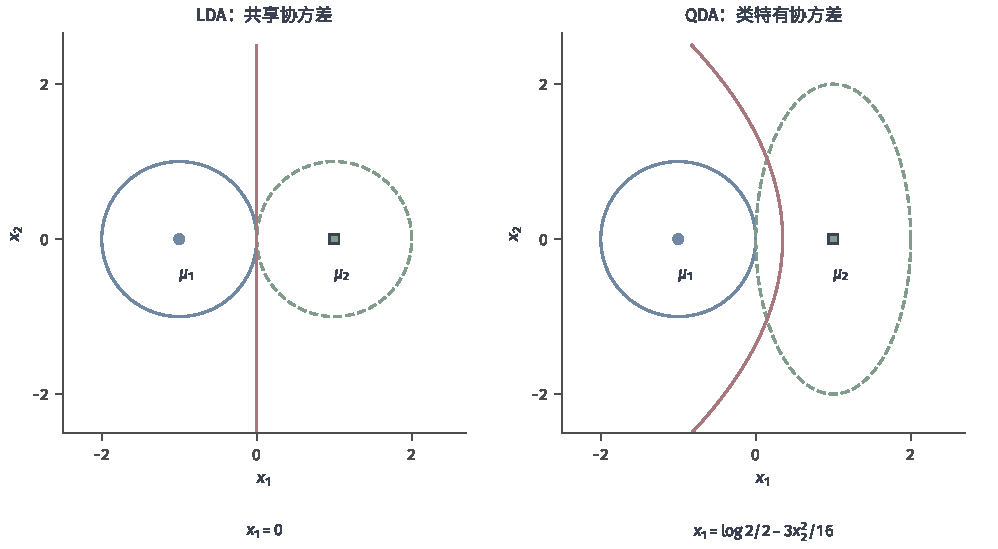
\includegraphics[width=159.059mm]{figures/04-classic-models/00-shared/matplotlib/classification-gaussian-boundaries/figure.pdf}
  \caption{两图均取$\pi_1=\pi_2=1/2$、$\bm{\mu}_1=(-1,0)^{\top}$、$\bm{\mu}_2=(1,0)^{\top}$和$\bm{\Sigma}_1=\bm{I}_2$，仅第2类协方差变化。蓝色圆点和绿色方点为均值，蓝色实线与绿色虚线分别为$\Delta_1=1$和$\Delta_2=1$的等密度轮廓；不同类的这些轮廓不保证密度值相同。红色粗线按$g_1=g_2$的解析式绘制，底部公式分别给出LDA的线性边界与QDA的二次边界。参数均为教学构造，不是采样或拟合结果。}
  \label{fig:classification-gaussian-boundaries}
\end{figure*}

对二分类，把式~\eqref{eq:classification-lda-score}~中的两类得分相减并归一化，就得到Logistic形式的后验。因此，共享高斯假设蕴含线性对数几率，反过来却不成立；许多非高斯输入分布也能有Logistic形式的条件概率。即便两条路线的后验形式相同，用联合似然估计均值和协方差，与直接最大化条件似然，也通常得到不同的有限样本参数。

完整协方差每类需要$d(d+1)/2$个自由参数。类内散布矩阵的秩至多为$n_c-1$，因而$n_c\leq d$时必然奇异，不能直接代入普通高斯密度；$n_c>d$也不保证估计准确或条件良好。共享估计的秩至多为$n-C$。在维数较大或类别样本少时，可以共享、取对角，或采用第\ref{sec:classification-lda-covariance-extensions}节的RDA收缩估计。式\eqref{eq:classification-rda}已经说明这些约束如何借用合并统计量和球形方差；使用收缩就改变了估计准则，不再是未经约束的MLE。

稠密完整协方差的统计成本约为$O(nd^2)$，各类矩阵分解约为$O(Cd^3)$，存储为$O(Cd^2)$，QDA单样本得分约为$O(Cd^2)$。LDA只需分解一份协方差，并可预先算出线性权重，使单样本预测降到$O(Cd)$。实现时可用Cholesky分解求解二次型与对数行列式，无须显式构造逆矩阵。

\subsection{模型对比与总结}
\label{sec:classification-probability-comparison}

Logistic与Softmax直接拟合类别条件概率，NB与GDA先拟合类先验和类条件输入分布。前者不必解释输入怎样产生，后者则可利用分布约束减少需要估计的关系。二分类Logistic是Softmax的两类形式；两者都以互斥类别为对象，多标签任务需要另行规定每个标签事件的模型。

高斯模型的关系由协方差约束决定：QDA允许各类独立的完整协方差，LDA要求共享，高斯NB要求各类协方差对角。LDA与高斯NB各自限制了不同对象，不能一般地按强弱排序。共享高斯模型的共同二次项在类别比较中相消，后验可写成线性Softmax；QDA则需要平方项和交叉项。为Softmax提供这些扩展特征可以表达QDA后验，却无需把系数解释为高斯密度参数。相同的后验形式也不意味着相同学习：联合似然估计与条件似然估计在有限样本上通常选出不同系数。

NB与线性Logistic的联系还取决于事件模型。参数严格为正时，伯努利NB的对数得分累加二值字段，多项式NB的得分按本节文档长度约定累加词项计数，其后验可以写成这些特征上的Softmax。高斯NB在各类单维方差不同时还含有平方项，只是没有跨坐标的交叉项。补集NB改变统计来源，AODE增加部分条件依赖；收缩协方差改变估计约束。这些变化应分别与具体数据缺口比较，不能一律解释成“概率模型更复杂”。

表\ref{tab:classification-probability-comparison}汇总相同监督分类任务下的主要取舍。参数量按每维分布参数有界计算，GDA的共享与类特有协方差分别列明，避免把两者的代价混在一起。
\begin{table}[htbp]
  \centering
  \small
  \begin{tabularx}{\linewidth}{@{}
    >{\RaggedRight\arraybackslash}p{0.19\linewidth}
    >{\RaggedRight\arraybackslash}X
    >{\RaggedRight\arraybackslash}X@{}}
    \toprule
    模型 & 建模与估计 & 主要取舍 \\
    \midrule
    Logistic回归／Softmax回归 &
    直接拟合条件概率；$O(Cd)$个参数，迭代优化 &
    不拟合输入分布；需检查特征表示、分离与正则化 \\
    NB &
    由先验和简化类条件模型形成后验；通常$O(Cd)$个参数 &
    计数或矩估计易累积；依赖和事件模型失配会引入偏差 \\
    共享GDA（LDA） &
    高斯类条件分布，共享协方差；$O(d^2+Cd)$个参数 &
    用共同协方差降低估计波动；只得到线性边界 \\
    类特有GDA（QDA） &
    各类独立估计协方差；$O(Cd^2)$个参数 &
    边界更灵活；对每类样本量和协方差条件更敏感 \\
    \bottomrule
  \end{tabularx}
  \caption{概率分类模型的建模对象与估计代价。所有概率输出都需单独检查校准，参数量不直接等于达到指定精度所需的样本量。}
  \label{tab:classification-probability-comparison}
\end{table}

类条件假设可以减轻小样本下的估计负担，也可能留下模型失配。Ng和Jordan对特定NB与判别式模型的研究展示了这种取舍，不能据此给全部生成式与判别式模型排序\scite{ng2001}。实际选择应固定输入表示、数据划分、误判代价和调参预算，比较分类错误、概率质量与计算成本；训练误差更小或输出取值合法，都不能单独说明概率已经可靠。
